% ------- Create Preamble ------------
\documentclass [12pt]{article} 
\usepackage[a4paper]{geometry} 
\usepackage{amsmath, amsthm, amssymb, amsfonts}
 \usepackage{graphicx,epsfig}
\usepackage{booktabs} 
\usepackage{pslatex} 
\usepackage{caption} 
\usepackage{setspace} 
\usepackage{hyperref} 
\usepackage{multicol, multirow}
\usepackage{graphicx,epsfig}
\usepackage{booktabs}
\usepackage{pslatex}
\usepackage{caption}
\usepackage{setspace}
\usepackage{hyperref}
\usepackage{multicol}
\usepackage{textgreek}
\usepackage{pdfpages}
\usepackage{apacite}
\usepackage{float}
\newtheorem{hypothesis}{Hypothesis}
\newtheorem{nullhypothesis}{Null Hypothesis}
\usepackage{tikz}
%---Set up author and title page
\singlespace
\title{The new kids are on the block: incentives for congressional caucuses to disregard seniority in leadership assignments}
\author{Damon C.\ Roberts\footnote{Ph.D Student,
Department of Political Science, University of Colorado Boulder, UCB 333, Boulder, CO 80309-0333. Damon.Roberts-1@colorado.edu.}}

%set up document
\date{}
\begin{document}
\maketitle
\begin{abstract}

Why might Congressional leaders seek to promote younger and fresher faces in their chambers to leadership positions? In this paper, I provide a theory suggesting that caucus leadership may seek to endorse newer members over those who have been in their respective chamber longer. I also suggest that the Democratic caucus has a unique incentive to also promote younger members. These incentives are all quite dependent on the electoral strengths that member brings to the table for the caucus as a whole. This argument further supports the literature suggesting strong partisan teamsmanship is ever present in the post-reform Congress and the parties are quite concerned with seeking electoral advantages for their members.

\end{abstract}

\newpage
\doublespace
\newpage 
\section*{Introduction}

% TODO Write the Introduction at the end %
The role of the seniority system in the textbook Congress received little attention despite the acute implications of its existence and the eventual institutional and political impacts of its formal removal by Congress in the 1970's \cite{Celler1961}. Since the House of Representatives formally moved away from the seniority system for Committee and other leadership positions, the continued research on the seniority system as an informal institution speaks to the role that it plays as an institution in its own right. The literature is quite well-developed and the scholars interested in studying these sets of questions have strongly 

As I later discuss, I argue that the literature of the seniority system needs to better 

Building on the existing literature of the seniority system and the motivations that drive legislator behavior in Congress, I argue that there are other incentives that party leaders may pursue that the seniority system cannot provide to the caucus. In this argument I assume that parties are important to Congress \cite<see>{Cox2005,Rohde1991a}. 

For some time now, scholars of the behavior of lawmakers have accepted that a key goal of officeholders is to be reelected and as a result, institutions are built to help members of Congress (heretofore abbreviated as MC's) realize that goal \cite{Mayhew1974}. As the Conditional Party Governance model proposed by \cite{Rohde1991a} contends, leaders have incentives to ensure that their party remains in the majority and that their members are reelected. To be reelected, MC's must provide some 

\section*{What Seniority Looks Like In The Post-Reform Era}

First, central to this theory and the assumptions contained within it is understanding the motivations of individual MC's who are likely working for their own self interest but also it is important to understand the motivations of party leaders who are primarily focused on their caucus and retaining and improving others' status. Before directly addressing the literature on the seniority system, I first am going to explicitly discuss the goals and motivations of members of congress to then move into how a responsible party allows for their members to achieve those to then explore how those motivations may inform the seniority system and how they tie into the existing literature.

\citeA{Mayhew1974} famously claimed that members of Congress seek reelection, above all else. Others have added that MC's also seek to increase their influence by seeking higher position and to make good public policy \cite{Fenno1973}. As a result, institutions are structured in ways to help protect these goals \cite{Mayhew1974}. By implication, MC's push and seek reforms that help them achieve the goal of reelection, by increasing their influence if they want to, and to make good public policy - or at least good for their district. These reforms need not be exclusive to formal rules but they can also be changes to the informal rules which may adjust the norms of the institution. For example, in the late $19^{th}$ century and early $20^{th}$ century, Congress saw a number of changes when "Boss" Reed and "Czar" Cannon shaped the relative power of the Speaker of the House. These adjustment to the norms and rules of the House were meant to centralize control over the House around the speaker. These two MC's when elected to the speaker of the House both sought to discipline those who were not loyal to them but also sought to control the agenda more than any other Speakers had done previously \cite{Cox2005}. Later reforms that helped MC's further achieve benefits was to make a series of reforms in the 1970's.

The House reforms in the 1970's have proven pivotal to shaping the political landscape we observe today. These reforms are also quite influential in scholarly debates about Congress as well. Scholars have long debated whether parties matter in Congress. \citeA{Mayhew1974} proposed a theory where MC's were individualistic and self-interested actors who did not gain much utility from aligning with their party and establishing a solid voting bloc with the other members. Some scholars pitched that parties act as useful voting coalitions that MC's use on some issues and in some contexts; but on some issues, MC's would have to look out for their district and their own interests and vote against their party at a non-trivial rate \cite{Aldrich}. Others who agreed with Mayhew's proposition that parties are not important claimed that pivotal voters in policy gridlock are what mattered; that parties had no power over correcting for gridlock \cite{Krehbiel1991}. 

In the post-reform era, scholars claim that parties have become stronger; largely as a result of the 1970 reforms. \citeA{Rohde1991a} for example claimed that in instances where members of a caucus agree, parties have an impact. That is, parties matter as a voting block to the degree to which there is homogeneity among its members. This Conditional Party Governance theory,  implies that if people agree with their fellow partisans on a particular vote, they are likely to work together as a cohesive unit. Other scholars joined this debate to say that parties matter quite a lot. While parties do not explicitly control and punish those who do not vote a particular way, parties skirt this problem by controlling the available options that are even put before the floor. This Procedural Cartel theory claims that parties seek to maintain their majority status when they have it \cite{Cox2005}. To do so, parties seek to help their members by pushing bills through that matter to their members' constituents and are crucial to seeing the most vulnerable achieve reelection \cite{Cox2005}. While doing this, parties achieve their collective goal - which is to increase the power of its members in Congress, while also assisting individuals realize their personal goals of reelection and an upward career trajectory \cite{Cox2005}. 

The Cartel Theory of parties in Congress provides a compelling starting point for studying the role of seniority. This theory implies that parties are powerful. It implies that members who seek to continue to have party support in their reelection campaigns, their ability to credit claim, their ability to tell their constituents about all of the successes they have representing their interests, need to have some amount of fealty to the party and its leadership. Those who continue to support the collective interest of the party and do their job to push fellow party members' policies within their committee assignment's jurisdiction will be rewarded and will find their job of achieving their individual goals much easier.

These incentives are quite clearly relevant for leadership assignments and seniority. After all, increasing one's relevance and power as a lawmaker begins with increasing one's seniority within the institution. Those who hold subcommittee and coveted committee chairperson titles have more influence in that they have more ability to claim the leadership positions and assignments that they want and may need for their constituents, they have more ability to control the agenda within their policy jurisdictions, and they can increasingly attach their names to other important politicians and issues that increase their district-level and national recognizability. 


While caucus members seek to help one another through the collective good, the current discussion has not yet addressed whether more senior representatives are actually useful to the caucus as a whole. Thankfully, scholars have addressed this question. Overall, it appears that the literature is somewhat skeptical that senior representatives are helpful for helping individual members get reelected and for the party to achieve a maintenance of majority status. As \citeA{Krehbiel1991} argues, seniority is a good thing in Congress - it increases information due to more expertise. That information can then be shared with the general membership and fellow partisans \cite{Krehbiel1991}. By implication, senior members are valuable to the extent that they use and share information to build legislative coalitions to pass effective policy \cite{Taylor2019}. From this, scholars studying the benefits of the seniority system claim that because of this ability to build legislative power are more popular among their constituents in their reelection bids and therefore provide more stability to the caucus leadership. Specifically, \citeA{McKelvey1992} finds that voters do not know or do not care about their representative's relative seniority but instead care about their ability to get things done in congress and whether their representative holds any legislative power to strike bargains. 

This line of work appears somewhat fraught. Scholars studying the origins information in Congress would imply that starting from the point of information as a key factor in support of seniority as a heuristic for assignments is incorrect. A number of scholars have argued that information comes from a number of places in and around Congress \cite{Austen-Smith1993,Hall2006,McCrain2018}. In line with this argument's implications for the seniority system \citeA{Ansolabehere2014} argue that seniority matters very little to voters; voters only care about whether their representative provide observable benefits to the district. Other work not looking at the seniority system support this idea that seniority and its benefits are not what provide stability in membership. For example, more ideologically extreme members tend to be more popular more recently than the moderate ones - those who are likely to have been in Congress longer \cite{Utych2019}. In agreement with \citeA{Ansolabehere2014}, \citeA{Kellermann2009} argue that seniority matters very little. In this instance, \citeA{Kellermann2009} come from the position of the bargaining power you may have to pass legislation rather than the electoral and stability benefits you provide to your caucus. Here, they argue that seniority only impacts the likelihood that you remain on your current committees and the extent to which you face challenges passing legislation in that committee's jurisdiction \cite{Kellermann2009}. That is, those who hold more senior roles on a variety of committees often will face more success at pushing bills through on those policy jurisdictions relative to those who are less senior but do not see any electoral advantages. Seniority, then, seems to be an individual benefit and not much of a collective one.

The literature has provided a useful foundation for which to build a theory of seniority's utility upon. The literature indicates a need to assume that parties are relatively strong and that the theory needs to consider a bargain between the party and the individual member. Parties, it seems, do not benefit in majority status retention from the seniority system. Instead, parties indirectly benefit in this way from the seniority of its members when those senior members effectively provide benefits to their constituents. The path between stability of the caucus' members do not directly come from seniority, but instead they must encourage and not stand in the way of senior members seeking to produce good policy that their constituents will benefit from. The literature also implies that the role of information and the ability to build a coalition is not very strong due to the effectiveness by which parties act as stable coalitions already for those seeking passage of a bill. Individual members who may be less senior, may seek party support and promotion by signaling to the party that they are effective legislators who will be reelected in the future and who aid other members in the caucus in their legislative pursuits. This all is to say that the literature indicates that senior members are not exclusively helpful for the parties. Senior members must have other attributes and signal these to the caucus. In the next section I provide a simple formal model \footnote{Unfortunately, my knowledge of the method is limited to that of a graduate student who was mediocre in an introductory graduate level game theory seminar.} to articulate my theory in a detailed and comprehensive way. 


\section*{Incentives For Caucus Leadership To Fink On Seniority}

To begin the discussion, I first outline a number of benefits an individual may bring to the caucus to convince them of their value in an assignment. The first benefit may be that individuals may bring electoral advantage to the caucus in a number of ways. The common thread for which they may do this is dependent on a demographic of voter that the party is vying for. For example, both parties seem to be vying for more ideologically extreme candidates in the House of Representatives. Some have argued and provided some empirical evidence indicating that more ideological candidates are more popular among the public, on both sides \cite{Utych2019}. Candidates may also be descriptively aligned with the party or their interests and may be alluring to the party in that way. 

A second benefit that candidates may provide is policy expertise from prior experience. Parties are not only concerned about reelecting their members. Good public policy is indirectly beneficial to electoral chances of caucus members but they also help build a platform for the party which may help grow the influence of the party across a number of offices at the state level and other levels of the Federal government such as the Senate or the Presidency. If a newly minted representative seeks an assignment and can demonstrate a deep wealth of knowledge for that assignment's jurisdiction, they may prove themselves to be an asset for the party. Moreover, this benefit of expertise increases once one considers how miserly MC's are when it comes to information as discussed in the review of the literature above. Therefore, prior experience with the policy, pre-established networks with bureaucrats or other policy experts, and knowledge about industry and economic reactions to policy implementation, are all benefits that come along with a member who has prior experience and knowledge with a particular policy area. 

These two leading benefits that caucuses may receive from finking on seniority have some powerful impacts on the decision making of assignments. Figure \ref{Fig1} demonstrates a very simple formal model including the payoffs included for both the caucus (l) and the individual member wanting an assignment (M) to begin in a bargain for the position they desire. The game starts with a nature node that specifies where on a continuum of probability that the member will be useful for the caucus as a policy and electoral maximizer ($\beta$). The party seeks a scenario wherein the party assigns leaders that maximizes the caucuses total available benefits: 
\begin{equation} \label{eq.1}
l_\beta = \DeclareMathOperator{argMax}{(\beta)}
\end{equation}


The individual member seeks the opposite scenario. They seek to provide just enough benefits to capture an assignment that they want:

\begin{equation} \label{eq.2}
M_\beta = \DeclareMathOperator{argMin}{(\beta)}
\end{equation}

With this established, we can derive a simple model to determine in what scenarios the bargain meets the conditions in Equations \ref{eq.1} and \ref{eq.2} to create an equilibrium.

\begin{figure}
% Node styles
\begin{center}

\tikzset{
% Two node styles for game trees: solid and hollow
solid node/.style={circle,draw,inner sep=1.5,fill=black},
hollow node/.style={circle,draw,inner sep=1.5,fill=white}

}

\begin{tikzpicture}[scale=1.5,font=\footnotesize] 

% Specify spacing for each level of the tree
\tikzstyle{level 1}=[level distance=15mm,sibling distance=15mm]
\tikzstyle{level 2}=[level distance=10mm,sibling distance=35mm]
\tikzstyle{level 3}=[level distance=10mm,sibling distance=12mm]
\tikzstyle{level 4}=[level distance=10mm,sibling distance=12mm]
% The Tree
\node(0)[solid node,label=above:{$N$}]{} 
child{node(1)[solid node, white]{}
}
child{[white] node(2)[solid node, yshift=-35]{$M$} %note that you need to adjust the yshift if you change the sibling distance
child{[black] node(4)[solid node, label=above:{$l$}]{} 
child{[black] node(6)[solid node, label=below:{$(\beta, 1)$}]{} edge from parent node[left]{$A$}}
child{[black] node(6)[solid node, label=below:{$(1-\delta,0 - d)$}]{} edge from parent node[left]{$\tilde A$}}
edge from parent node[left]{$C$}
}
child{[black] node(5)[solid node, label=below:{$(1-\delta, 0)$}]{}
edge from parent node[right]{$\tilde C$}
}
 edge from parent node[black, xshift=0,yshift=-42]{$\beta\epsilon[0,1]$} %note that you need to adjust the yshift if you change the level distance
}
child{node(3)[solid node, white]{}
}; 

% information set
    \draw[bend right](1)to(3);
\end{tikzpicture}
\caption{Incentives for finking on seniority system}	 
\label{Fig1}
\end{center}
\end{figure}

Figure \ref{Fig1} presents the payoff structure where $N$ dictates what benefits ($\beta$) the individual member, $M$, provides to the caucus, $l$. $M$, knowing the value of $\beta$ may choose to either campaign, $C$, or to not campaign, $\tilde C$. If $M$ chooses $\tilde C$, then it is likely due to the fact that they know they cannot meet the minimum requirement, $\beta^*$, that $l$ requires to even consider them for a position. If they do not campaign, which is certainly suboptimal for $M$ since they get nothing from this scenario if they are interested in leadership positions. Likewise, $l$ does not lose too much from this situation, either. They are left with some uncertainty, $\delta$, as to how well the alternative selections for the assignment are in providing a high $\beta$; however, this is the status quo that $l$ is accustomed to. 

More interestingly, we see the subgame where $M$ chooses $C$. In this condition, the value of $\beta$ is crucially important given the assumption communicated in Equations \ref{eq.1} and \ref{eq.2}. In the scenario where $\beta$ equals or it is asymptotically 0, $\lim_{\beta\to\ 0$, and $M$ still chooses $C$, then it is likely that $l$ will select the status quo, which is to reject, $\tilde A$, $M$'s offer and $M$ gets $0-d$, the status quo with some reputational cost, $d$. In a scenario where $\lim_{\beta\to\ 1$, then $l$ is likely to accept $M$'s offer and both get what they want; they meet the conditions in Equations \ref{eq.1} and \ref{eq.2}. The balance of the game lies in $\beta$. This indicates that $M$ must credibly demonstrate $\beta$. In most cases, seniority acts as the signal as to whether $M$ credibly possess enough benefits. When $M$ believes that they likely meet $l$'s needs, $\beta^*$, then this is the scenario whereby $M$ is most likely to choose $C$ and make an offer. Otherwise, when $M$ does not meet $l$'s requirement of $\beta^*$, then $M$ is likely to choose the status quo which is to $\tilde C$ as compared to the status quo with some reputational costs for wasting the leadership and the caucuses' time for offering a leadership role that they are ill-equipped for. 

The game demonstrates a couple of interesting phenomenon. The first is that the seniority system is certainly preferred over finking on it. In most cases, $M$ and $l$ prefer to uphold and support the status quo. Second, the game demonstrates that the power is held within $l$. $M$ has power to the extent that they can control and correctly signal $\beta$, which is not very much when they have just ascended to office. The game does demonstrate, though, that more experienced and professional politicians and lawmakers are what spark a deviation from the status quo. This supports prevailing hypotheses that many MC's are increasingly seeking a career in politics. It also demonstrates that having characteristics for which the party wants, is a sufficient but increasingly necessary condition for new politicians to become more influential in the House of Representatives. As discussed earlier in the paper, these could be ideological extremity, being young or a minority if you are a Democrat, being staunchly socially conservative as we saw with the Republicans and the Tea Party Movement, as examples. 

\section*{Empirical Evidence for Reduction in Seniority}

My formal model sought to detail a comprehensive theory to the incentive structure for individual members of congress and for those of the caucuses' interest via proxy of the leadership. It is quite challenging to test this theory empirically. Unlike the work studying American political attitudes and behavior, I am limited to observational data only; I am unable to collect and utilize data which provide information about the motivations of the nation's top politicians. Any data that are available are observational and are, at best, inferential. To not spend too much time on analyzing data which are limited, my claim here is that these data are not support for my theory. Rather, these data are descriptive and intend to demonstrate whether some of the assumptions I make in my game theoretic model have any empirical founding.

Congressional Seniority is commonly measured based on an MC's term length. To study empirical evidence of my theory's assumptions I first, I use data from the Brookings Institute's Vital Statistics on Congress. These data provide information about the average term length of all MC's in that given session. The summary data are presented in the first figure below.

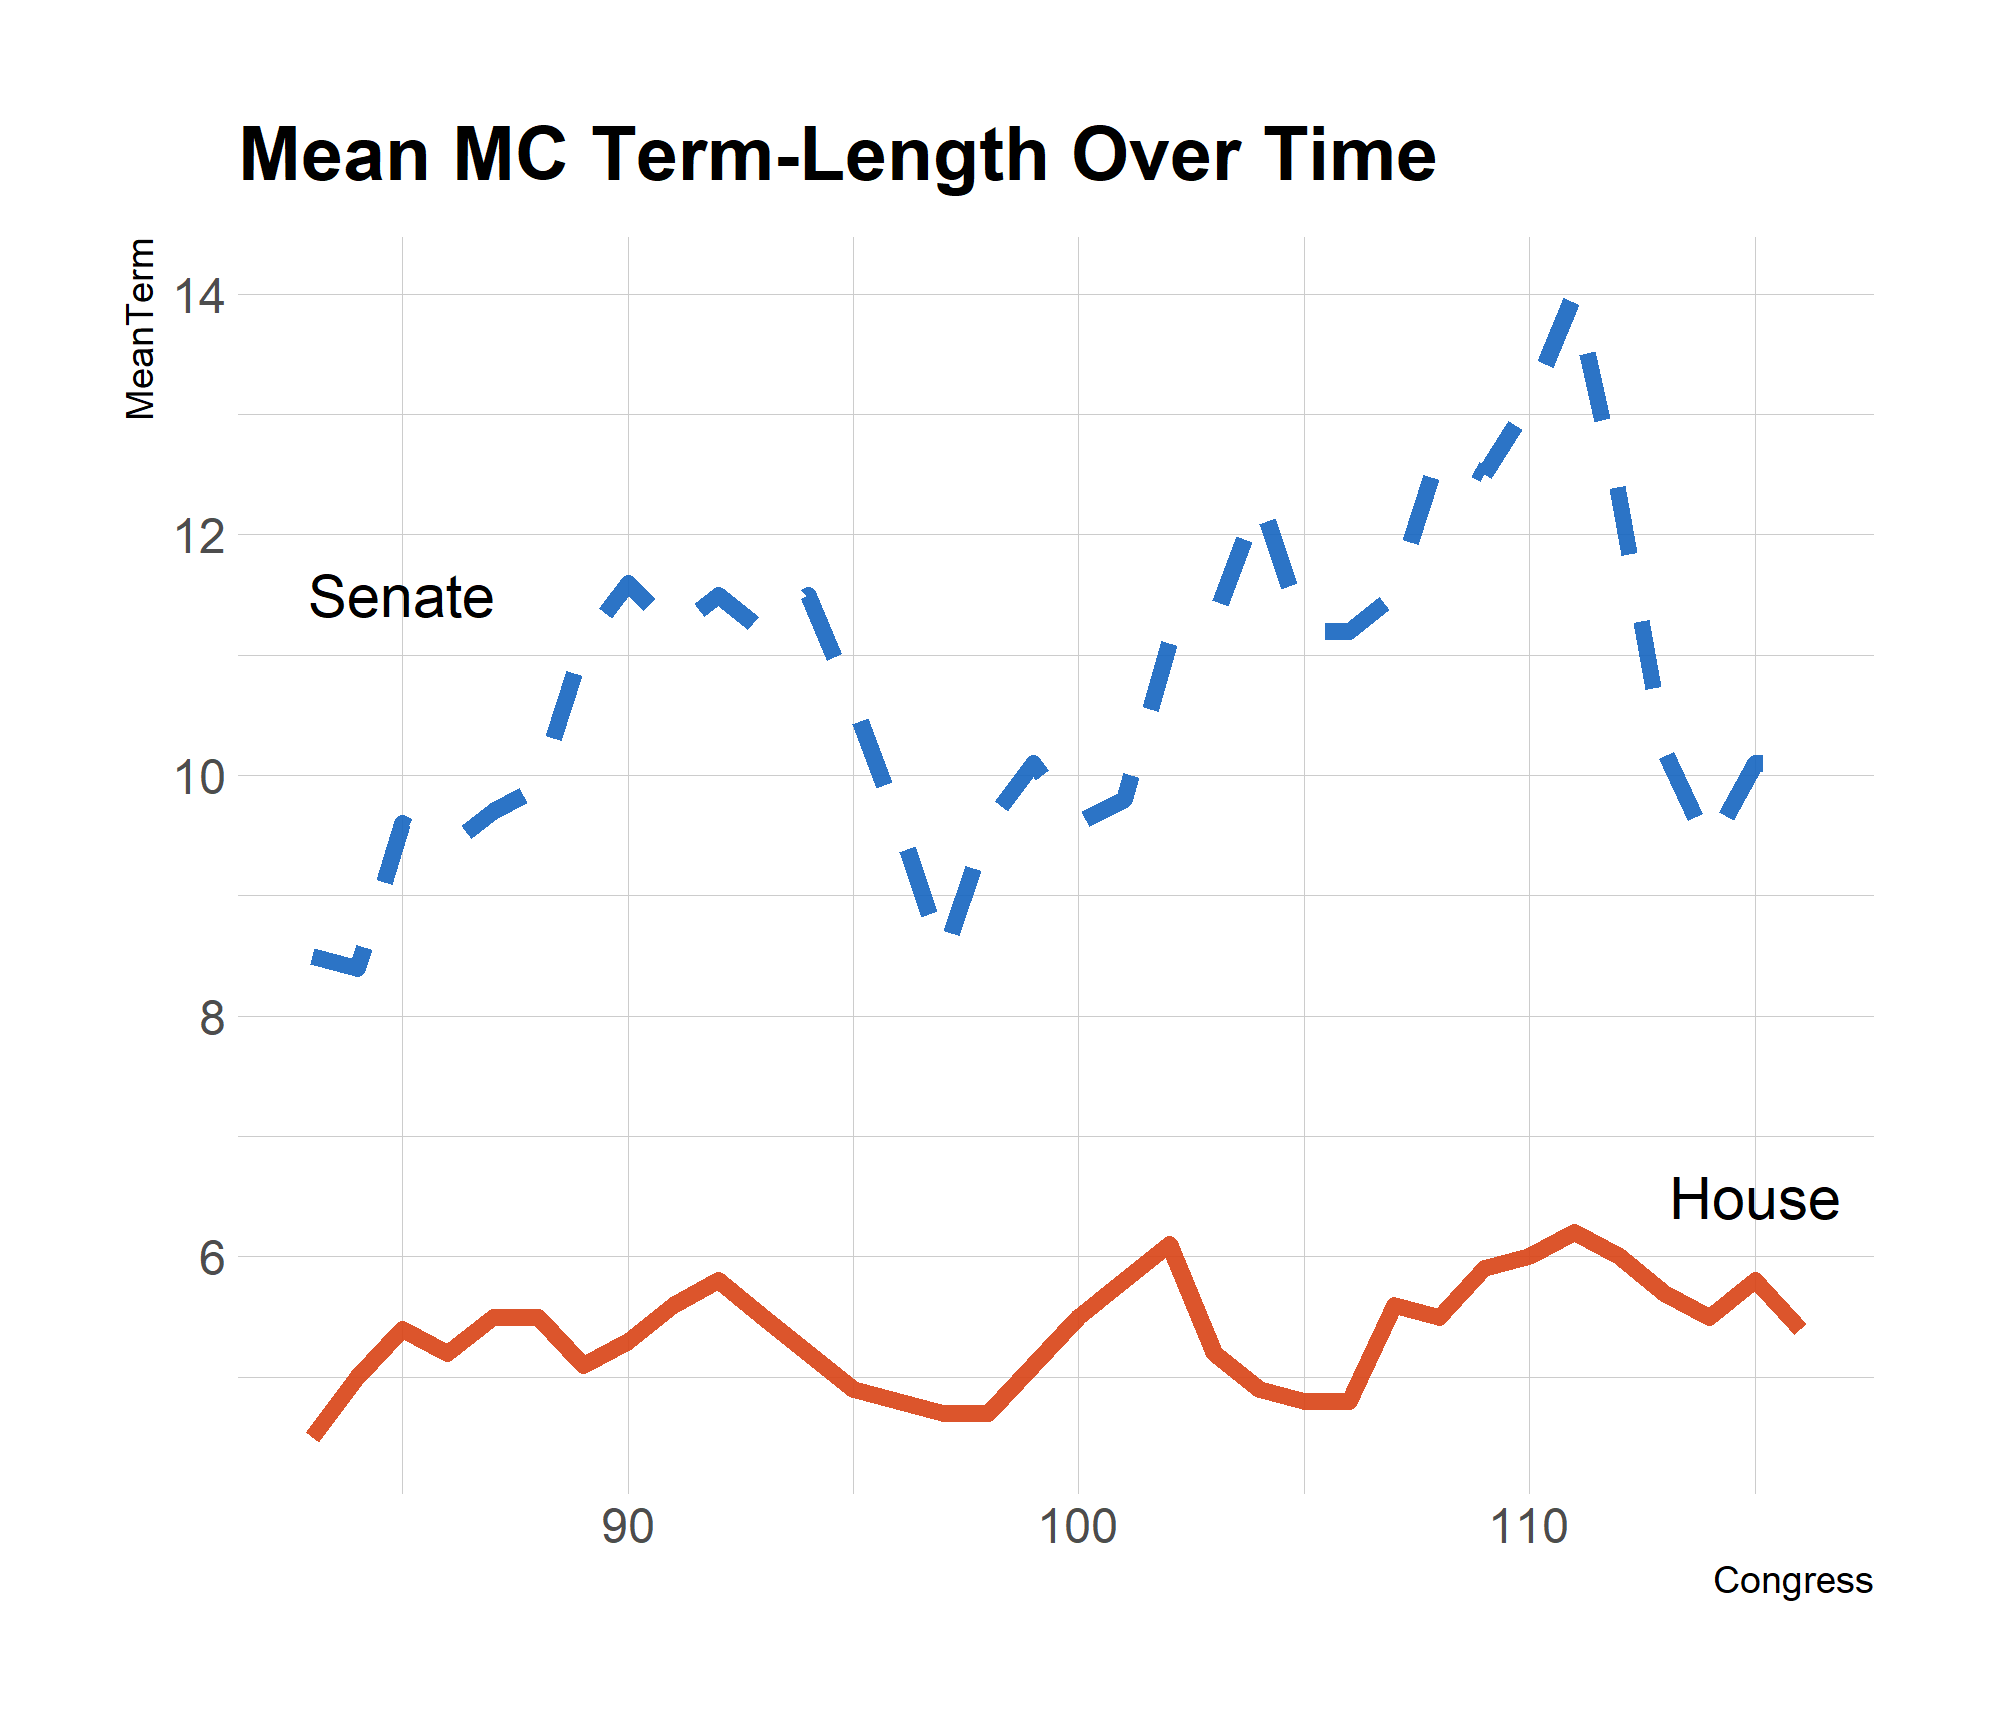
\includegraphics[height=250, width=400]{../figures/term-time-plot.png}

Here we see that in more recent sessions, overall, MC's are spending less time in office. Unsurprisingly, we see that Senator's are spending more time in Congress. This plot does not account for the 6 years senators have in Congress as compared to the 2-year terms representatives have. Term length is not the only important measure related to expertise and experience in my game theoretic model; age is a relevant proxy for academic, nonprofit, and agency experience. For example, It may be the case that a younger MC may be treated differently than an older but no-more senior colleague. 

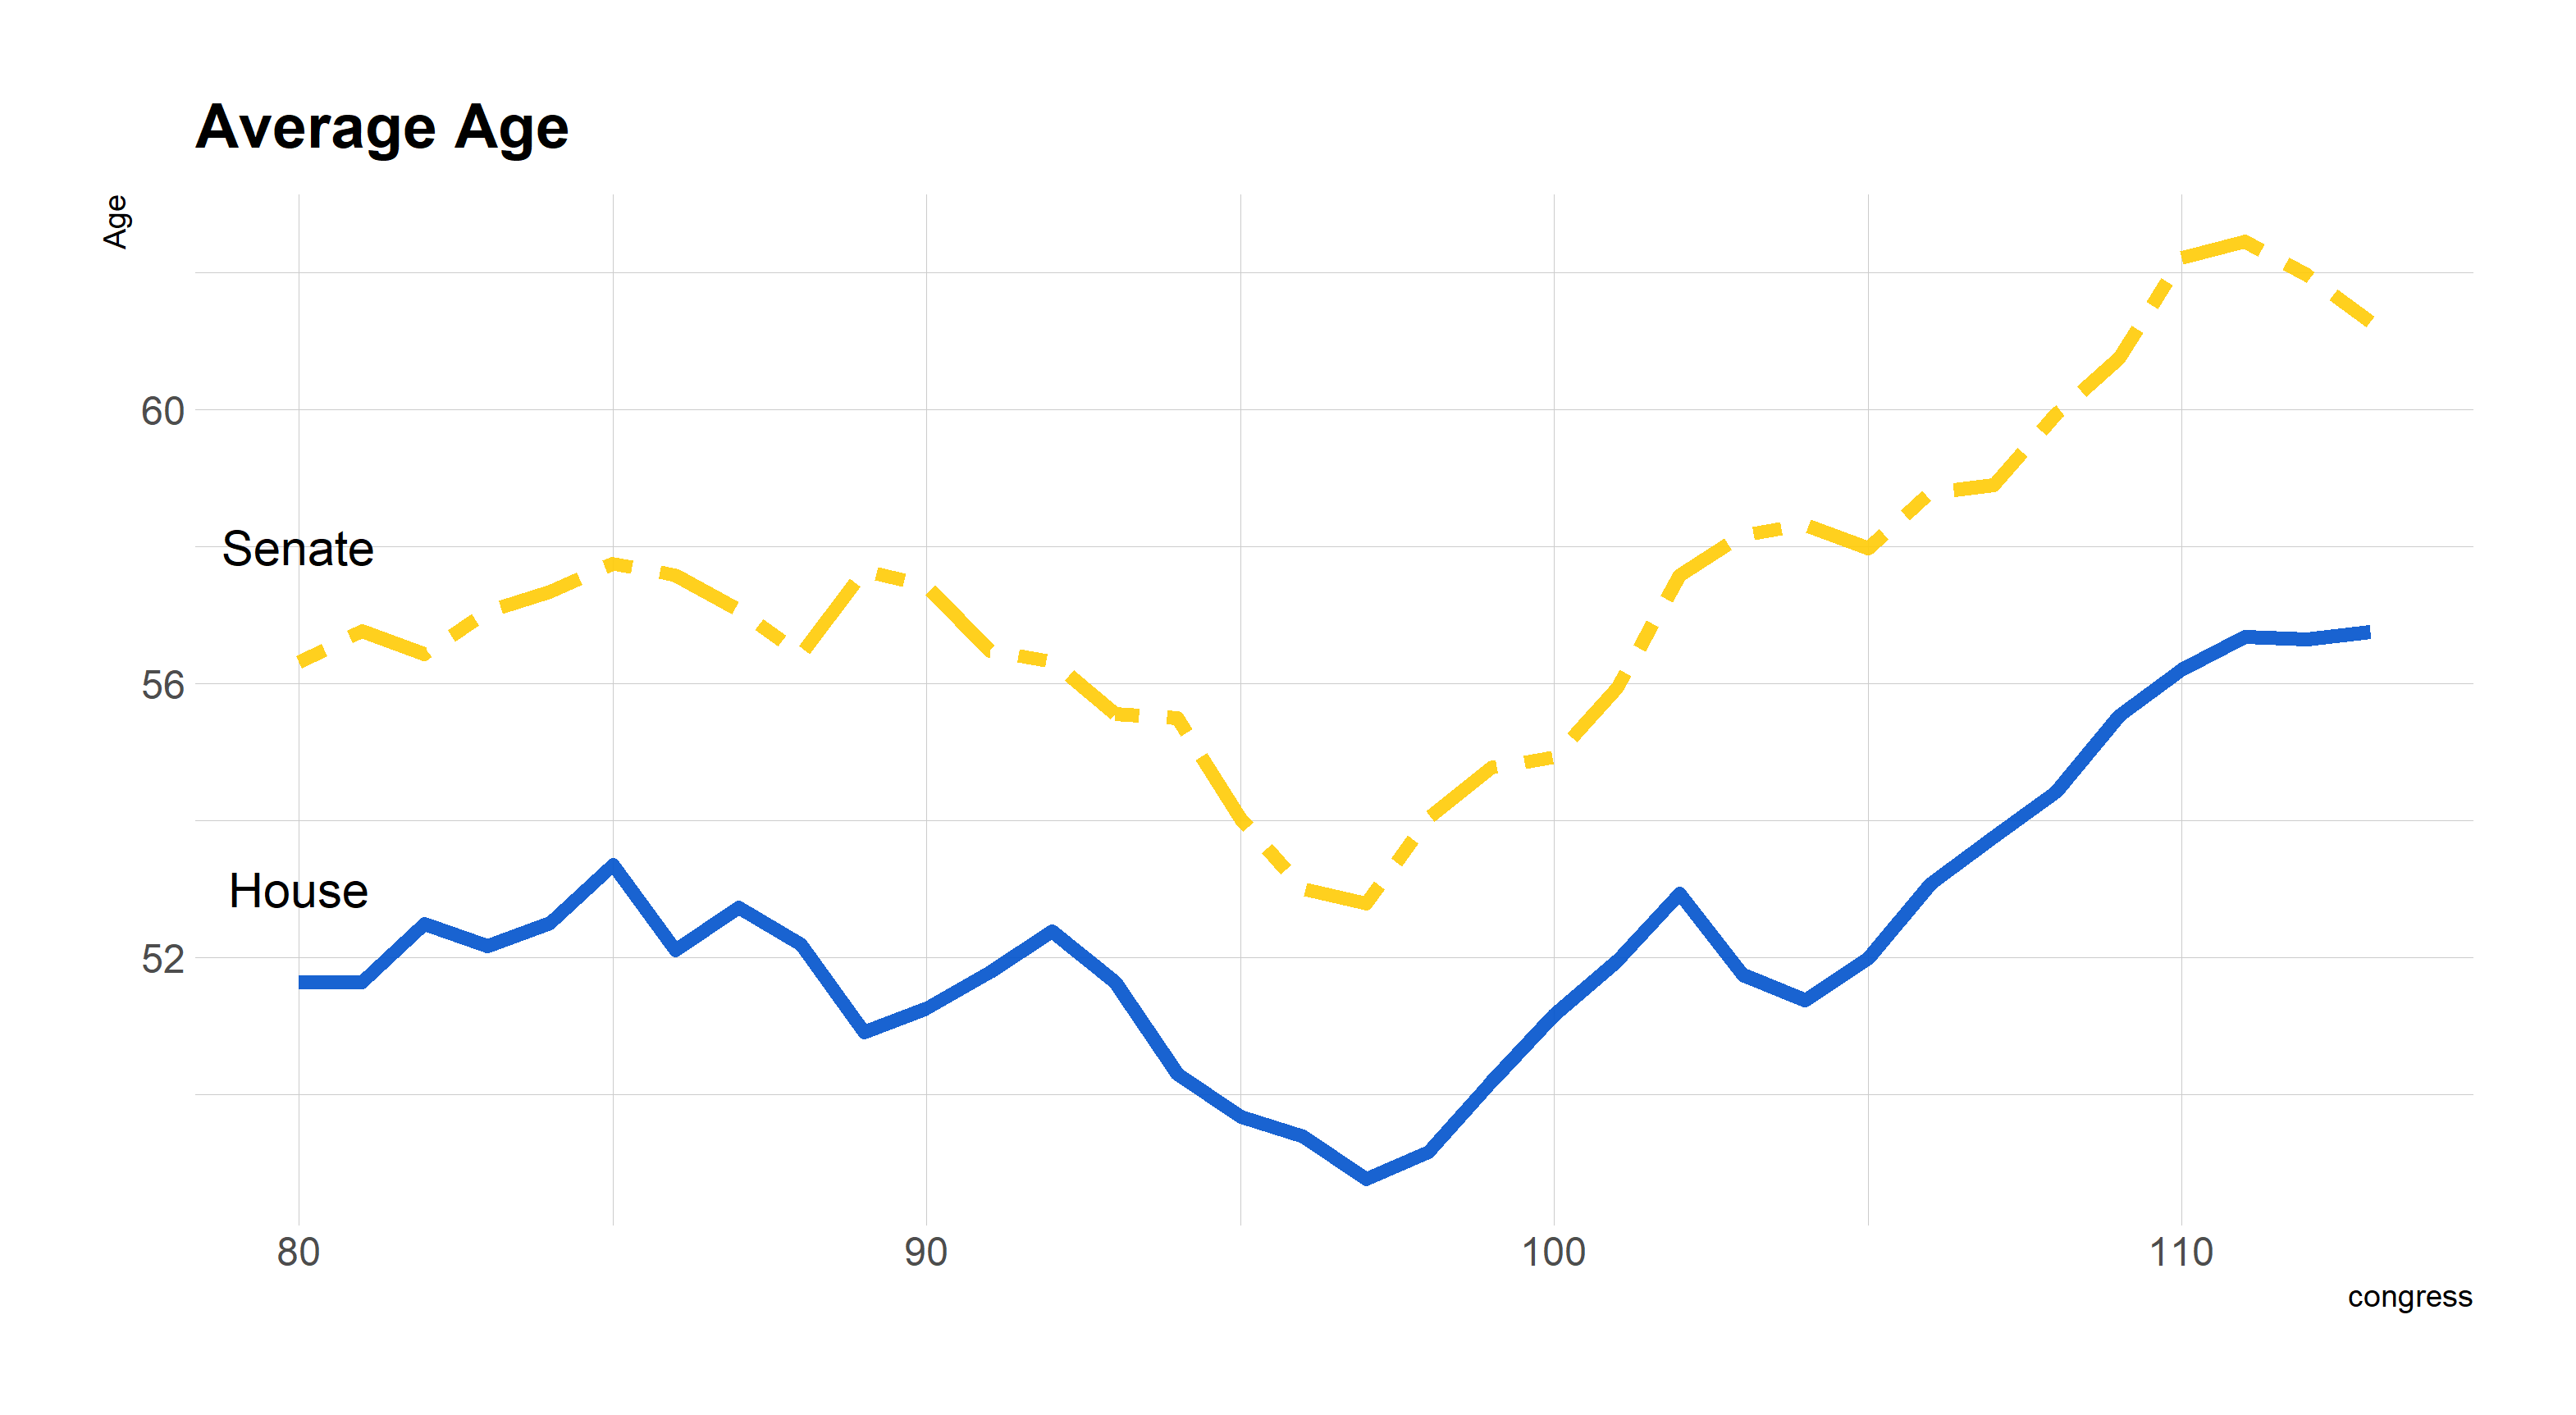
\includegraphics[height=250, width=400]{../figures/age-over-time}

The second figure presents data from FiveThirtyEight's Congress Age project. The data are the average of all MC's in each chamber for that given session. We see that over time, MC's have become older. There appears to be a small inflection point near the end of FiveThirtyEight's dataset demonstrating there was a session or two that have been a bit younger.

These figures so far only demonstrate the demographics of the entire Congress and does not focus on the members holding leadership positions. To most explicitly determine whether the use of seniority has decreased over time, I use Volden and Wiseman's data on the U.S. House that runs from the 1970's until the 2018 Congress. With that data, I subset my dataset to only include those in leadership positions (subcommittee or committee Chairs, Majority or Minority Leadership - as defined by Volden and Wiseman, or whether they held an Appropriation's Committee seat) for that particular session of Congress. I then calculated how many years that member had been in Congress based on the first year of the session they took office and the first year of the current term. To be transparent, this is still a descriptive analysis and is not multivariate. This means that I did not control for any factors nor did I conduct any tests or corrections for the stationarity of the data - this is not an empirical model and is not correlational. The third figure presents a plot of these data.

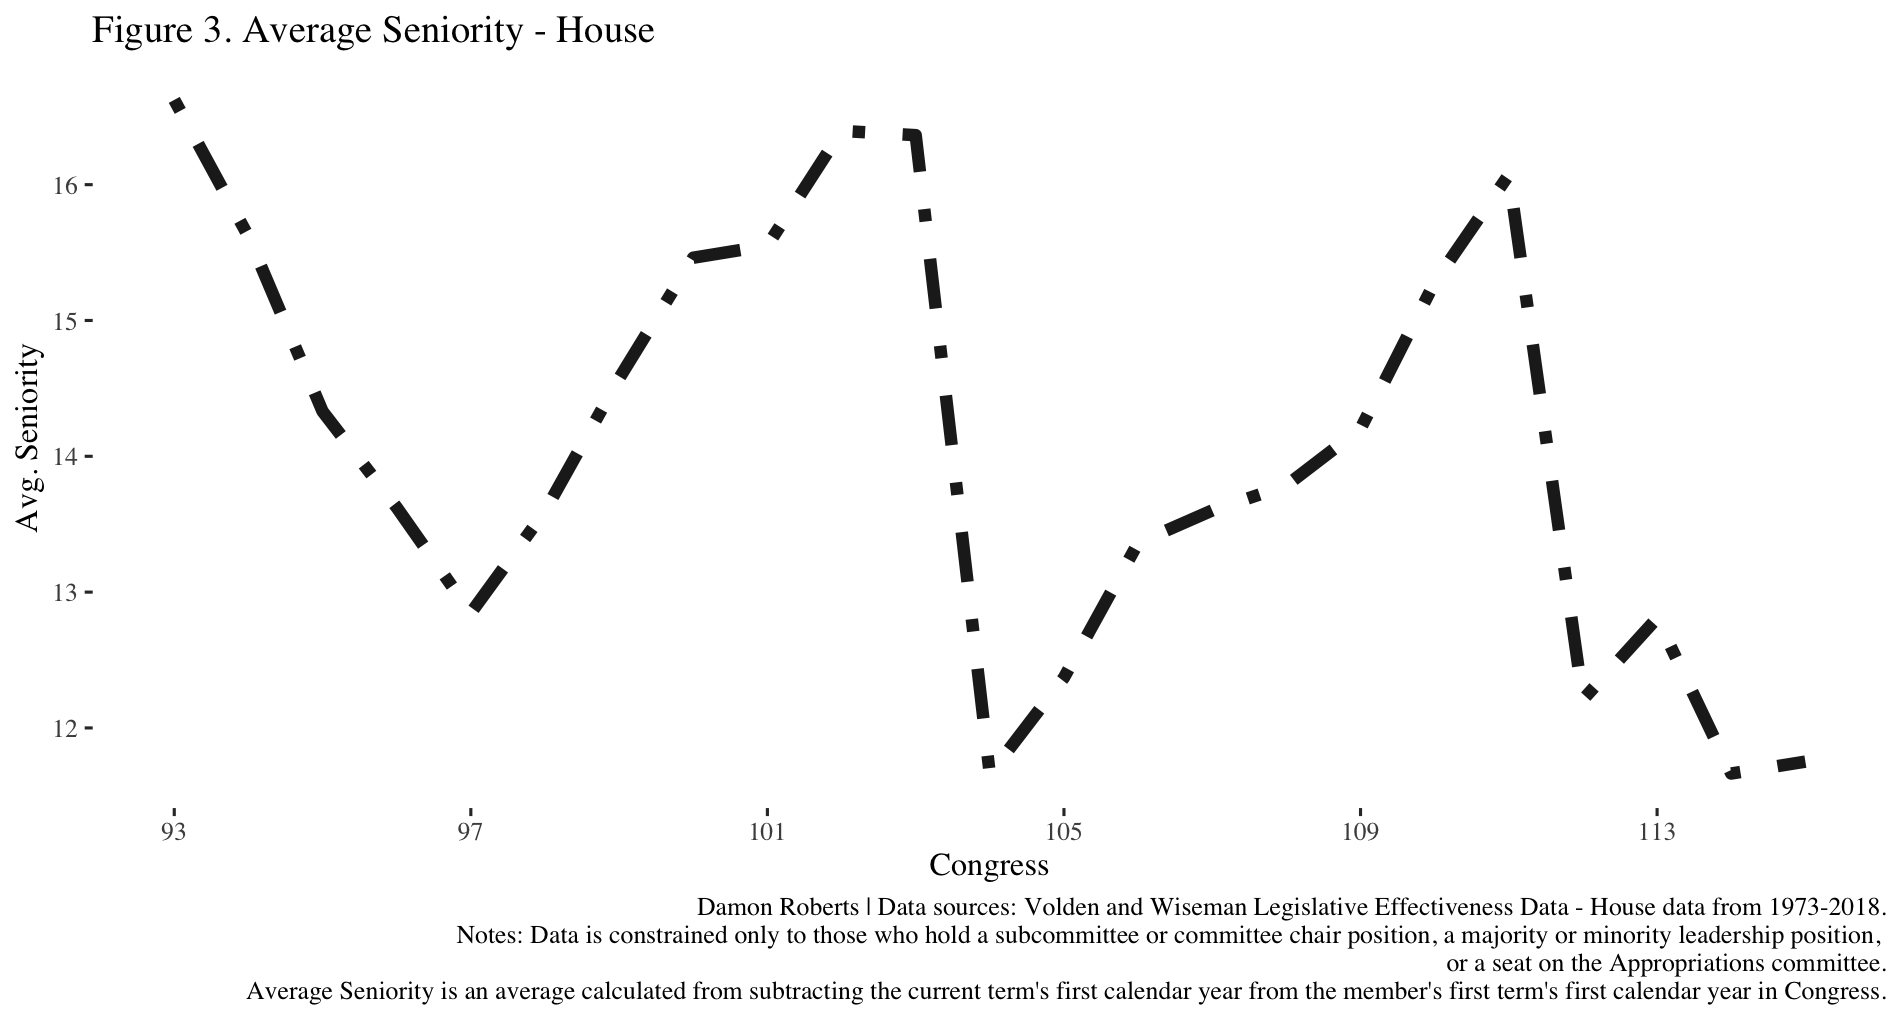
\includegraphics[height=250,width=400]{../figures/avg-house-seniority-macro.png}

These descriptive data demonstrate that there is a downward trend in holding any leadership position and the number of years on has been in office in the House of Representatives. This graphic, while simple, provides some descriptive evidence that scholarly efforts to an increased attention of Congressional assignments are warrented. Specifically, it presents some basic evidence that there might not be a perfect correlation between seniority and leadership assignment and perhaps this correlation is decreasing over time as well. This figure also demonstrates that a claim of plausibly statistically significant alternative explanations besides seniority for leadership assignment in the House has empirical support. 

It is important here to not conflate the number of terms with seniority violations, however. To be sure to not overstate the takeaways a reader should have from the figure, it the differences between seniority and term length should be identified before moving on. When scholars operationalize seniority, they are referring to the length of time \textit{within} the committee or subcommittee and not overall length of time in the chamber. The figure presented here, presents time in the chamber and not within assignments. This is one of the key challenges with quantifying the seniority system - the need to identify violations of seniority within subcommittees and committees as opposed to using the more widely available data on the chambers as a whole. 

\section*{Discussion and Conclusion}

Observing that seniority has decreased in the House of Representatives since the 1970's among those holding leadership positions despite a much more stable trend of term length of the average member of Congress and an increasing age of the average member of Congress, this indicates a need for further scholarly exploration of the incentives a majority caucus may pursue as an alternative to within caucus seniority. 

In this paper, I argue that there are in fact a number of interesting alternative incentives and a resulting bargaining structure that guide the majority caucus' decision for leadership assignments. Specifically, I argue, in line with the common conclusion from the Rubenstein infinite-horizon solution concept, that the bargain between individual members wanting a leadership role and the caucus needs to find an equilibrium that at least guarantees reelection for the individual member and a loyalty to their copartisan colleagues to yield positive benefits for their colleague's reelection bids. This condition requires that the individual member commits to support policy within the leadership candidate's committee jurisdiction to ensure that their colleague's policies pass and they can maximize relevant incumbency advantages such as the ability to claim credit to their constituents.

This bargain implies a strong interdependence among copartisan colleagues for the realization of their career goals. This model also more centrally associates the informal seniority system with the motivations first discussed by \citeA{Fenno1973} and \citeA{Mayhew1974}.  

\newpage
\bibliographystyle{apacite}
\bibliography{/Users/damonroberts/Dropbox/Bibliographies/Krehbiel1991,/Users/damonroberts/Dropbox/Bibliographies/Celler1961,/Users/damonroberts/Dropbox/Bibliographies/Mayhew1974,/Users/damonroberts/Dropbox/Bibliographies/Cox2005,/Users/damonroberts/Dropbox/Bibliographies/Rhode1991a,/Users/damonroberts/Dropbox/Bibliographies/Fenno1973,/Users/damonroberts/Dropbox/Bibliographies/Aldrich,/Users/damonroberts/Dropbox/Bibliographies/McKelvey1992,/Users/damonroberts/Dropbox/Bibliographies/Taylor2019,/Users/damonroberts/Dropbox/Bibliographies/Austen-Smith1993,/Users/damonroberts/Dropbox/Bibliographies/Hall2006,/Users/damonroberts/Dropbox/Bibliographies/McCrain2018,/Users/damonroberts/Dropbox/Bibliographies/Ansolabehere2014,/Users/damonroberts/Dropbox/Bibliographies/Utych2019,/Users/damonroberts/Dropbox/Bibliographies/Kellermann2009}
\end{document}